\documentclass[
	letterpaper, % Paper size, specify a4paper (A4) or letterpaper (US letter)
	10pt, % Default font size, specify 10pt, 11pt or 12pt
]{CSUniSchoolLabReport}

%----------------------------------------------------------------------------------------
%	REPORT INFORMATION
%----------------------------------------------------------------------------------------

\title{Lab Three\\ Fundamentals of Electronics \\ EECE2412/3} % Report title

\author{Michael \textsc{Brodskiy}\\ \small \href{mailto:Brodskiy.M@Northeastern.edu}{Brodskiy.M@Northeastern.edu}}

\date{October 29, 2024} % Date of the report

%----------------------------------------------------------------------------------------


\begin{document}

\maketitle % Insert the title, author and date using the information specified above

\begin{center}
	\begin{tabular}{l r}
		Date Performed: & October 15/22, 2024 \\ % Date the experiment was performed
        Partner: & Rahul \textsc{Singh} \\ % Partner names
		Instructor: & Professor \textsc{Onabajo} \\ % Instructor/supervisor
        TAs: & Ming \textsc{Xiang} \& Amr \textsc{Kassab} \\ % Teachers Assistants 
	\end{tabular}
\end{center}

\newpage

\begin{abstract}

  The goal of this laboratory experiment is to orient the performing individual with bipolar junction transistors (BJTs). Common regions (active, saturated, and cut-off) are explored, in addition to the effects of temperature variance on BJT performance. Finally, a light-emitting diode (LED) light-sensing circuit is constructed with a photocell. 

\end{abstract}

\begin{flushleft}

  \textsc{Keywords:} \underline{BJT}, \underline{active}, \underline{saturated}, \underline{cut-off}, \underline{temperature variance}, \underline{LED}, \underline{photocell}

\end{flushleft}

\newpage

\tableofcontents
\listoffigures

\newpage

\section{Equipment}

Available equipment included:\\

\begin{itemize}

  \item 2N3904 Bipolar Junction Transistors

  \item Light-Emitting Diodes (varying colors)

  \item Basic Circuit Components (Wires, Inductors, Capacitors, etc.)

  \item Keysight EDU36311A Dual DC Power Supply

  \item Photocell (Light-Varying Resistor)

\end{itemize}

\newpage

\section{Experimental Procedure}

We begin by constructing the following circuit:

\begin{figure}[H]
  \centering
  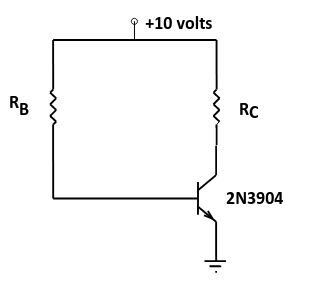
\includegraphics[width=.7\textwidth]{Figures/L3F1}
  \caption{BJT Biasing Circuit}
  \label{fig:1}
\end{figure}

We proceed to test various configurations which place the 2N3904 in common regions, such as active, saturated, and cut-off.

\subsection{The Forward-Active Region (with varying $\beta$)}

Using the circuit shown in Figure \ref{fig:1}, with $R_B=316.7[\si{\kilo\ohm}]$ and $R_C=1.003[\si{\kilo\ohm}]$, we place the BJT into its active region (supporting calculations are present in the pre-lab). Measuring $V_{CE}$ and $V_{BE}$ for both of our BJTs, we find:

$$V_{BE_1}=.708[\si{\volt}]\quad\text{ and }\quad V_{CE_1}=3.394[\si{\volt}]$$
$$V_{BE_2}=.704[\si{\volt}]\quad\text{ and }\quad V_{CE_2}=3.378[\si{\volt}]$$

We know the BJT is in its active region since, based on the above measurements, $V_{CE}>V_{BE}$ (or, alternatively $V_{BE}>0$ and $V_{BC}<0$).

Using the data from above, we may calculate $I_B$, $I_C$, and $\beta$:

$$I_{B_1}=\frac{10-.708}{316.7k}\quad\text{ and }\quad I_{C_1}=\frac{10-3.394}{1003}$$
$$\boxed{I_{B_1}=29.34[\si{\micro\ampere}]\quad\text{ and }\quad I_{C_1}=6.586[\si{\milli\ampere}]}$$

$$I_{B_2}=\frac{10-.704}{316.7k}\quad\text{ and }\quad I_{C_1}=\frac{10-3.378}{1003}$$
$$\boxed{I_{B_1}=29.353[\si{\micro\ampere}]\quad\text{ and }\quad I_{C_1}=6.6022[\si{\milli\ampere}]}$$

From this, we find the direct current (DC) gains:

$$\beta_1=\frac{6.586}{.02934}$$
$$\boxed{\beta_1=224.47}$$

$$\beta_2=\frac{6.6022}{.029353}$$
$$\boxed{\beta_2=224.92}$$

\subsubsection{Using Curve Tracers}

Per the curve tracer presented in class, we would expect $I_B=40[\si{\micro\ampere}]$ for our $I_C$ value. This gives us a $\beta$ of:

$$\beta_{curve}=\frac{6}{.04}$$
$$\boxed{\beta_{curve}=150}$$

\subsubsection{Tolerance and Standard Deviation of Gain}

It would be difficult to design a circuit with $\beta=150\pm 1\%$ because, even within the same model of BJT, there is much variation; however, it should still be practical to meet this strict tolerance. This is further supported by the variance of $\beta$ presented in the BJT data sheets attached to the laboratory experiment. Though the tested transistors are all within specification, there is a great amount of variance, which we can calculate using the standard deviation. We obtain two of each $\beta$ value from other groups:

$$\beta_1=186,196$$
$$\beta_2=201,217$$

The average of the gains is:

$$\beta_1^{avg}=202.16$$
$$\beta_2^{avg}=214.31$$

Thus, we get standard deviations of:

$$\boxed{\sigma_{\beta_1}=19.96\quad\text{ and }\sigma_{\beta_2}=12.185}$$

We may see that these standard deviations are all, more or less, within $1\%$ (for $\beta_1$ it is above for two of the three values), and, therefore, we should be able to design for such a tolerance.

\subsubsection{Thermal Response}

Using a can of refrigerant, we obtain new values:

$$V_{CE}=3.78[\si{\volt}]\quad\text{ and }\quad V_{BE}=.725[\si{\volt}]$$

This gives us:

$$\beta=\frac{\left( \frac{10-3.78}{1003} \right)}{\left( \frac{10-.725}{316700} \right)}$$
$$\boxed{\beta_{cold}=211.48}$$

Per the data sheets, we would expect a drop in $I_C$, which would result in a decrease in $\beta$, as shown above. This would be unwanted in a car stereo system, as colder weather would mean that the amplification would not be as great, thus causing lower volumes.

\subsection{BJT Saturation}

As per the pre-lab, we know that $R_B\leq 208.66[\si{\kilo\ohm}]$ will saturate the BJT. Thus, we select the closest available value: $R_B=157[\si{\kilo\ohm}]$. Measuring the saturation values, we find:

$$V_{CE_1}^{sat}=45[\si{\milli\volt}]\quad\text{ and }\quad V_{BE_1}^{sat}=.906[\si{\volt}]$$
$$V_{CE_2}^{sat}=51.5[\si{\milli\volt}]\quad\text{ and }\quad V_{BE_1}^{sat}=.94[\si{\volt}]$$

We see that there is a lot of variation between even the same model of BJT, and, thus, it is necessary to account for BJT-to-BJT variation. We may find the $\beta$ values for this region:

$$I_{B_1}=\frac{10-.906}{157000}\quad\text{ and }\quad I_{C_1}=\frac{10-.045}{1003}$$
$$\boxed{I_{B_1}=57.92[\si{\micro\ampere}]\quad\text{ and }\quad I_{C_1}=9.925[\si{\milli\ampere}]}$$

$$I_{B_2}=\frac{10-.94}{157000}\quad\text{ and }\quad I_{C_2}=\frac{10-.0515}{1003}$$
$$\boxed{I_{B_1}=57.7[\si{\micro\ampere}]\quad\text{ and }\quad I_{C_1}=9.9187[\si{\milli\ampere}]}$$

This gives us:

$$\beta_1=\frac{9.925}{.05792}$$
$$\boxed{\beta_1=171.36}$$

$$\beta_2=\frac{9.9187}{.0577}$$
$$\boxed{\beta_2=171.90}$$

From this, we see that, if a high $\beta$ is important in a circuit, we want to operate in the active, and not in the saturated region.

\subsection{BJT Cut-Off}

Using the different methods provided, we obtain:

$$V_{CE_1}=10[\si{\volt}]$$
$$V_{CE_2}=9.638[\si{\volt}]$$
$$V_{CE_3}=4.572[\si{\volt}]\quad\text{ (when $R=470[\si{\ohm}]$)}$$

\subsection{BJT Touch-Sensitive Switch}

\section{Conclusion}

\end{document}
